%-----------------------------------------------------------------------------------------------------------------------------------------------%
%	The MIT License (MIT)
%
%	Copyright (c) 2019 Jan Küster
%
%	Permission is hereby granted, free of charge, to any person obtaining a copy
%	of this software and associated documentation files (the "Software"), to deal
%	in the Software without restriction, including without limitation the rights
%	to use, copy, modify, merge, publish, distribute, sublicense, and/or sell
%	copies of the Software, and to permit persons to whom the Software is
%	furnished to do so, subject to the following conditions:
%	
%	THE SOFTWARE IS PROVIDED "AS IS", WITHOUT WARRANTY OF ANY KIND, EXPRESS OR
%	IMPLIED, INCLUDING BUT NOT LIMITED TO THE WARRANTIES OF MERCHANTABILITY,
%	FITNESS FOR A PARTICULAR PURPOSE AND NONINFRINGEMENT. IN NO EVENT SHALL THE
%	AUTHORS OR COPYRIGHT HOLDERS BE LIABLE FOR ANY CLAIM, DAMAGES OR OTHER
%	LIABILITY, WHETHER IN AN ACTION OF CONTRACT, TORT OR OTHERWISE, ARISING FROM,
%	OUT OF OR IN CONNECTION WITH THE SOFTWARE OR THE USE OR OTHER DEALINGS IN
%	THE SOFTWARE.
%	
%
%-----------------------------------------------------------------------------------------------------------------------------------------------%


%============================================================================%
%
%	DOCUMENT DEFINITION
%
%============================================================================%

%we use article class because we want to fully customize the page and don't use a cv template
\documentclass[10pt,A4]{article}	


%----------------------------------------------------------------------------------------
%	ENCODING
%----------------------------------------------------------------------------------------

% we use utf8 since we want to build from any machine
\usepackage[utf8]{inputenc}		

%----------------------------------------------------------------------------------------
%	LOGIC
%----------------------------------------------------------------------------------------

% provides \isempty test
\usepackage{xstring, xifthen}

%----------------------------------------------------------------------------------------
%	FONT BASICS
%----------------------------------------------------------------------------------------

% some tex-live fonts - choose your own

%\usepackage[defaultsans]{droidsans}
%\usepackage[default]{comfortaa}
%\usepackage{cmbright}
\usepackage[default]{raleway}
%\usepackage{fetamont}
%\usepackage[default]{gillius}
%\usepackage[light,math]{iwona}
%\usepackage[thin]{roboto} 

% set font default
\renewcommand*\familydefault{\sfdefault} 	
\usepackage[T1]{fontenc}

% more font size definitions
\usepackage{moresize}

%----------------------------------------------------------------------------------------
%	FONT AWESOME ICONS
%---------------------------------------------------------------------------------------- 

% include the fontawesome icon set
\usepackage{fontawesome}

% use to vertically center content
% credits to: http://tex.stackexchange.com/questions/7219/how-to-vertically-center-two-images-next-to-each-other
\newcommand{\vcenteredinclude}[1]{\begingroup
\setbox0=\hbox{\includegraphics{#1}}%
\parbox{\wd0}{\box0}\endgroup}

% use to vertically center content
% credits to: http://tex.stackexchange.com/questions/7219/how-to-vertically-center-two-images-next-to-each-other
\newcommand*{\vcenteredhbox}[1]{\begingroup
\setbox0=\hbox{#1}\parbox{\wd0}{\box0}\endgroup}

% icon shortcut
\newcommand{\icon}[3] { 							
	\makebox(#2, #2){\textcolor{maincol}{\csname fa#1\endcsname}}
}	

% icon with text shortcut
\newcommand{\icontext}[4]{ 						
	\vcenteredhbox{\icon{#1}{#2}{#3}}  \hspace{2pt}  \parbox{0.9\mpwidth}{\textcolor{#4}{#3}}
}

% icon with website url
\newcommand{\iconhref}[5]{ 						
    \vcenteredhbox{\icon{#1}{#2}{#5}}  \hspace{2pt} \href{#4}{\textcolor{#5}{#3}}
}

% icon with email link
\newcommand{\iconemail}[5]{ 						
    \vcenteredhbox{\icon{#1}{#2}{#5}}  \hspace{2pt} \href{mailto:#4}{\textcolor{#5}{#3}}
}

%----------------------------------------------------------------------------------------
%	Deutsche Silbentrennung
%----------------------------------------------------------------------------------------


\usepackage[ngerman]{babel}
\hyphenpenalty=10000



%----------------------------------------------------------------------------------------
%	PAGE LAYOUT  DEFINITIONS
%----------------------------------------------------------------------------------------

% page outer frames (debug-only)
% \usepackage{showframe}		

% we use paracol to display breakable two columns
\usepackage{paracol}

% define page styles using geometry
\usepackage[a4paper]{geometry}

% remove all possible margins
\geometry{top=1cm, bottom=1cm, left=1cm, right=1cm}

\usepackage{fancyhdr}
\pagestyle{empty}

% space between header and content
% \setlength{\headheight}{0pt}

% indentation is zero
\setlength{\parindent}{0mm}

%----------------------------------------------------------------------------------------
%	TABLE /ARRAY DEFINITIONS
%---------------------------------------------------------------------------------------- 

% extended aligning of tabular cells
\usepackage{array}

% custom column right-align with fixed width
% use like p{size} but via x{size}
\newcolumntype{x}[1]{%
>{\raggedleft\hspace{0pt}}p{#1}}%


%----------------------------------------------------------------------------------------
%	GRAPHICS DEFINITIONS
%---------------------------------------------------------------------------------------- 

%for header image
\usepackage{graphicx}

% use this for floating figures
% \usepackage{wrapfig}
% \usepackage{float}
% \floatstyle{boxed} 
% \restylefloat{figure}

%for drawing graphics		
\usepackage{tikz}				
\usetikzlibrary{shapes, backgrounds,mindmap, trees}

%----------------------------------------------------------------------------------------
%	Color DEFINITIONS
%---------------------------------------------------------------------------------------- 
\usepackage{transparent}
\usepackage{color}

% primary color
\definecolor{maincol}{RGB}{ 225, 0, 0 }

% accent color, secondary
% \definecolor{accentcol}{RGB}{ 250, 150, 10 }

% dark color
\definecolor{darkcol}{RGB}{ 70, 70, 70 }

% light color
\definecolor{lightcol}{RGB}{245,245,245}


% Package for links, must be the last package used
\usepackage[hidelinks]{hyperref}

% returns minipage width minus two times \fboxsep
% to keep padding included in width calculations
% can also be used for other boxes / environments
\newcommand{\mpwidth}{\linewidth-\fboxsep-\fboxsep}
	


%============================================================================%
%
%	CV COMMANDS
%
%============================================================================%

%----------------------------------------------------------------------------------------
%	 CV LIST
%----------------------------------------------------------------------------------------

% renders a standard latex list but abstracts away the environment definition (begin/end)
\newcommand{\cvlist}[1] {
	\begin{itemize}{#1}\end{itemize}
}

%----------------------------------------------------------------------------------------
%	 CV TEXT
%----------------------------------------------------------------------------------------

% base class to wrap any text based stuff here. Renders like a paragraph.
% Allows complex commands to be passed, too.
% param 1: *any
\newcommand{\cvtext}[1] {
	\begin{tabular*}{1\mpwidth}{p{0.98\mpwidth}}
		\parbox{1\mpwidth}{#1}
	\end{tabular*}
}

%----------------------------------------------------------------------------------------
%	CV SECTION
%----------------------------------------------------------------------------------------

% Renders a a CV section headline with a nice underline in main color.
% param 1: section title
\newcommand{\cvsection}[1] {
	\vspace{14pt}
	\cvtext{
		\textbf{\LARGE{\textcolor{darkcol}{\uppercase{#1}}}}\\[-4pt]
		\textcolor{maincol}{ \rule{0.1\textwidth}{2pt} } \\
	}
}

%----------------------------------------------------------------------------------------
%	META SKILL
%----------------------------------------------------------------------------------------

% Renders a progress-bar to indicate a certain skill in percent.
% param 1: name of the skill / tech / etc.
% param 2: percent, values range from 0 to 1
\newcommand{\cvskill}[2] {
	\begin{tabular*}{1\mpwidth}{p{0.72\mpwidth}  r}
 		\textcolor{black}{\textbf{#1}}\\
	\end{tabular*}%
	
	\hspace{4pt}
	\begin{tikzpicture}[scale=1,rounded corners=2pt,very thin]
		\fill [lightcol] (0,0) rectangle (1\mpwidth, 0.15);
		\fill [maincol] (0,0) rectangle (#2\mpwidth, 0.15);
  	\end{tikzpicture}%
}


%----------------------------------------------------------------------------------------
%	 CV EVENT
%----------------------------------------------------------------------------------------

% Renders a table and a paragraph (cvtext) wrapped in a parbox (to ensure minimum content
% is glued together when a pagebreak appears).
% Additional Information can be passed in text or list form (or other environments).
% the work you did
% param 1: time-frame i.e. Sep 14 - Jan 15 etc.
% param 2:	 event name (job position etc.)
% param 3: Customer, Employer, Industry
% param 4: Short description
\newcommand{\cvevent}[4] {
	
	% we wrap this part in a parbox, so title and description are not separated on a pagebreak
	% if you need more control on page breaks, remove the parbox
	\parbox{\mpwidth}{
		\begin{tabular*}{1\mpwidth}{p{0.72\mpwidth}  r}
	 		\textcolor{black}{\textbf{#2}} & \colorbox{maincol}{\makebox[0.25\mpwidth]{\textcolor{white}{#1}}} \\
			\textcolor{maincol}{\textbf{#3}} & \\
		\end{tabular*}\\[8pt]
	
		\ifthenelse{\isempty{#4}}{}{
			\cvtext{#4}\\
		}
	}

	\vspace{14pt}
}

%----------------------------------------------------------------------------------------
%	 CV META EVENT
%----------------------------------------------------------------------------------------

% Renders a CV event on the sidebar
% param 1: title
% param 2: subtitle (optional)
% param 3: customer, employer, etc,. (optional)
% param 4: info text (optional)
\newcommand{\cvmetaevent}[4] {
	\textcolor{maincol} {\cvtext{\textbf{\begin{flushleft}#1\end{flushleft}}}}

	\ifthenelse{\isempty{#2}}{}{
	\textcolor{darkcol} {\cvtext{\textbf{#2}} }
	}

	\ifthenelse{\isempty{#3}}{}{
		\cvtext{{ \textcolor{darkcol} {#3} }}\\
	}

	\cvtext{#4}\\[14pt]
}

%----------------------------------------------------------------------------------------
%	 About ME META EVENT
%----------------------------------------------------------------------------------------

% Renders a CV event on the sidebar
% param 1: info text (optional)
\newcommand{\aboutmemetaevent}[1] {

	\cvtext{#1}\\[14pt]
}

%---------------------------------------------------------------------------------------
%	QR CODE
%----------------------------------------------------------------------------------------

% Renders a qrcode image (centered, relative to the parentwidth)
% param 1: percent width, from 0 to 1
\newcommand{\cvqrcode}[1] {
	\begin{center}
		
\includegraphics[width={#1}\mpwidth]{frame}
	\end{center}
}


%============================================================================%
%
%
%
%	DOCUMENT CONTENT
%
%
%
%============================================================================%
\begin{document}
\columnratio{0.31}
\setlength{\columnsep}{2.2em}
\setlength{\columnseprule}{4pt}
\colseprulecolor{lightcol}
\begin{paracol}{2}
\begin{leftcolumn}
%---------------------------------------------------------------------------------------
%	META IMAGE
%----------------------------------------------------------------------------------------
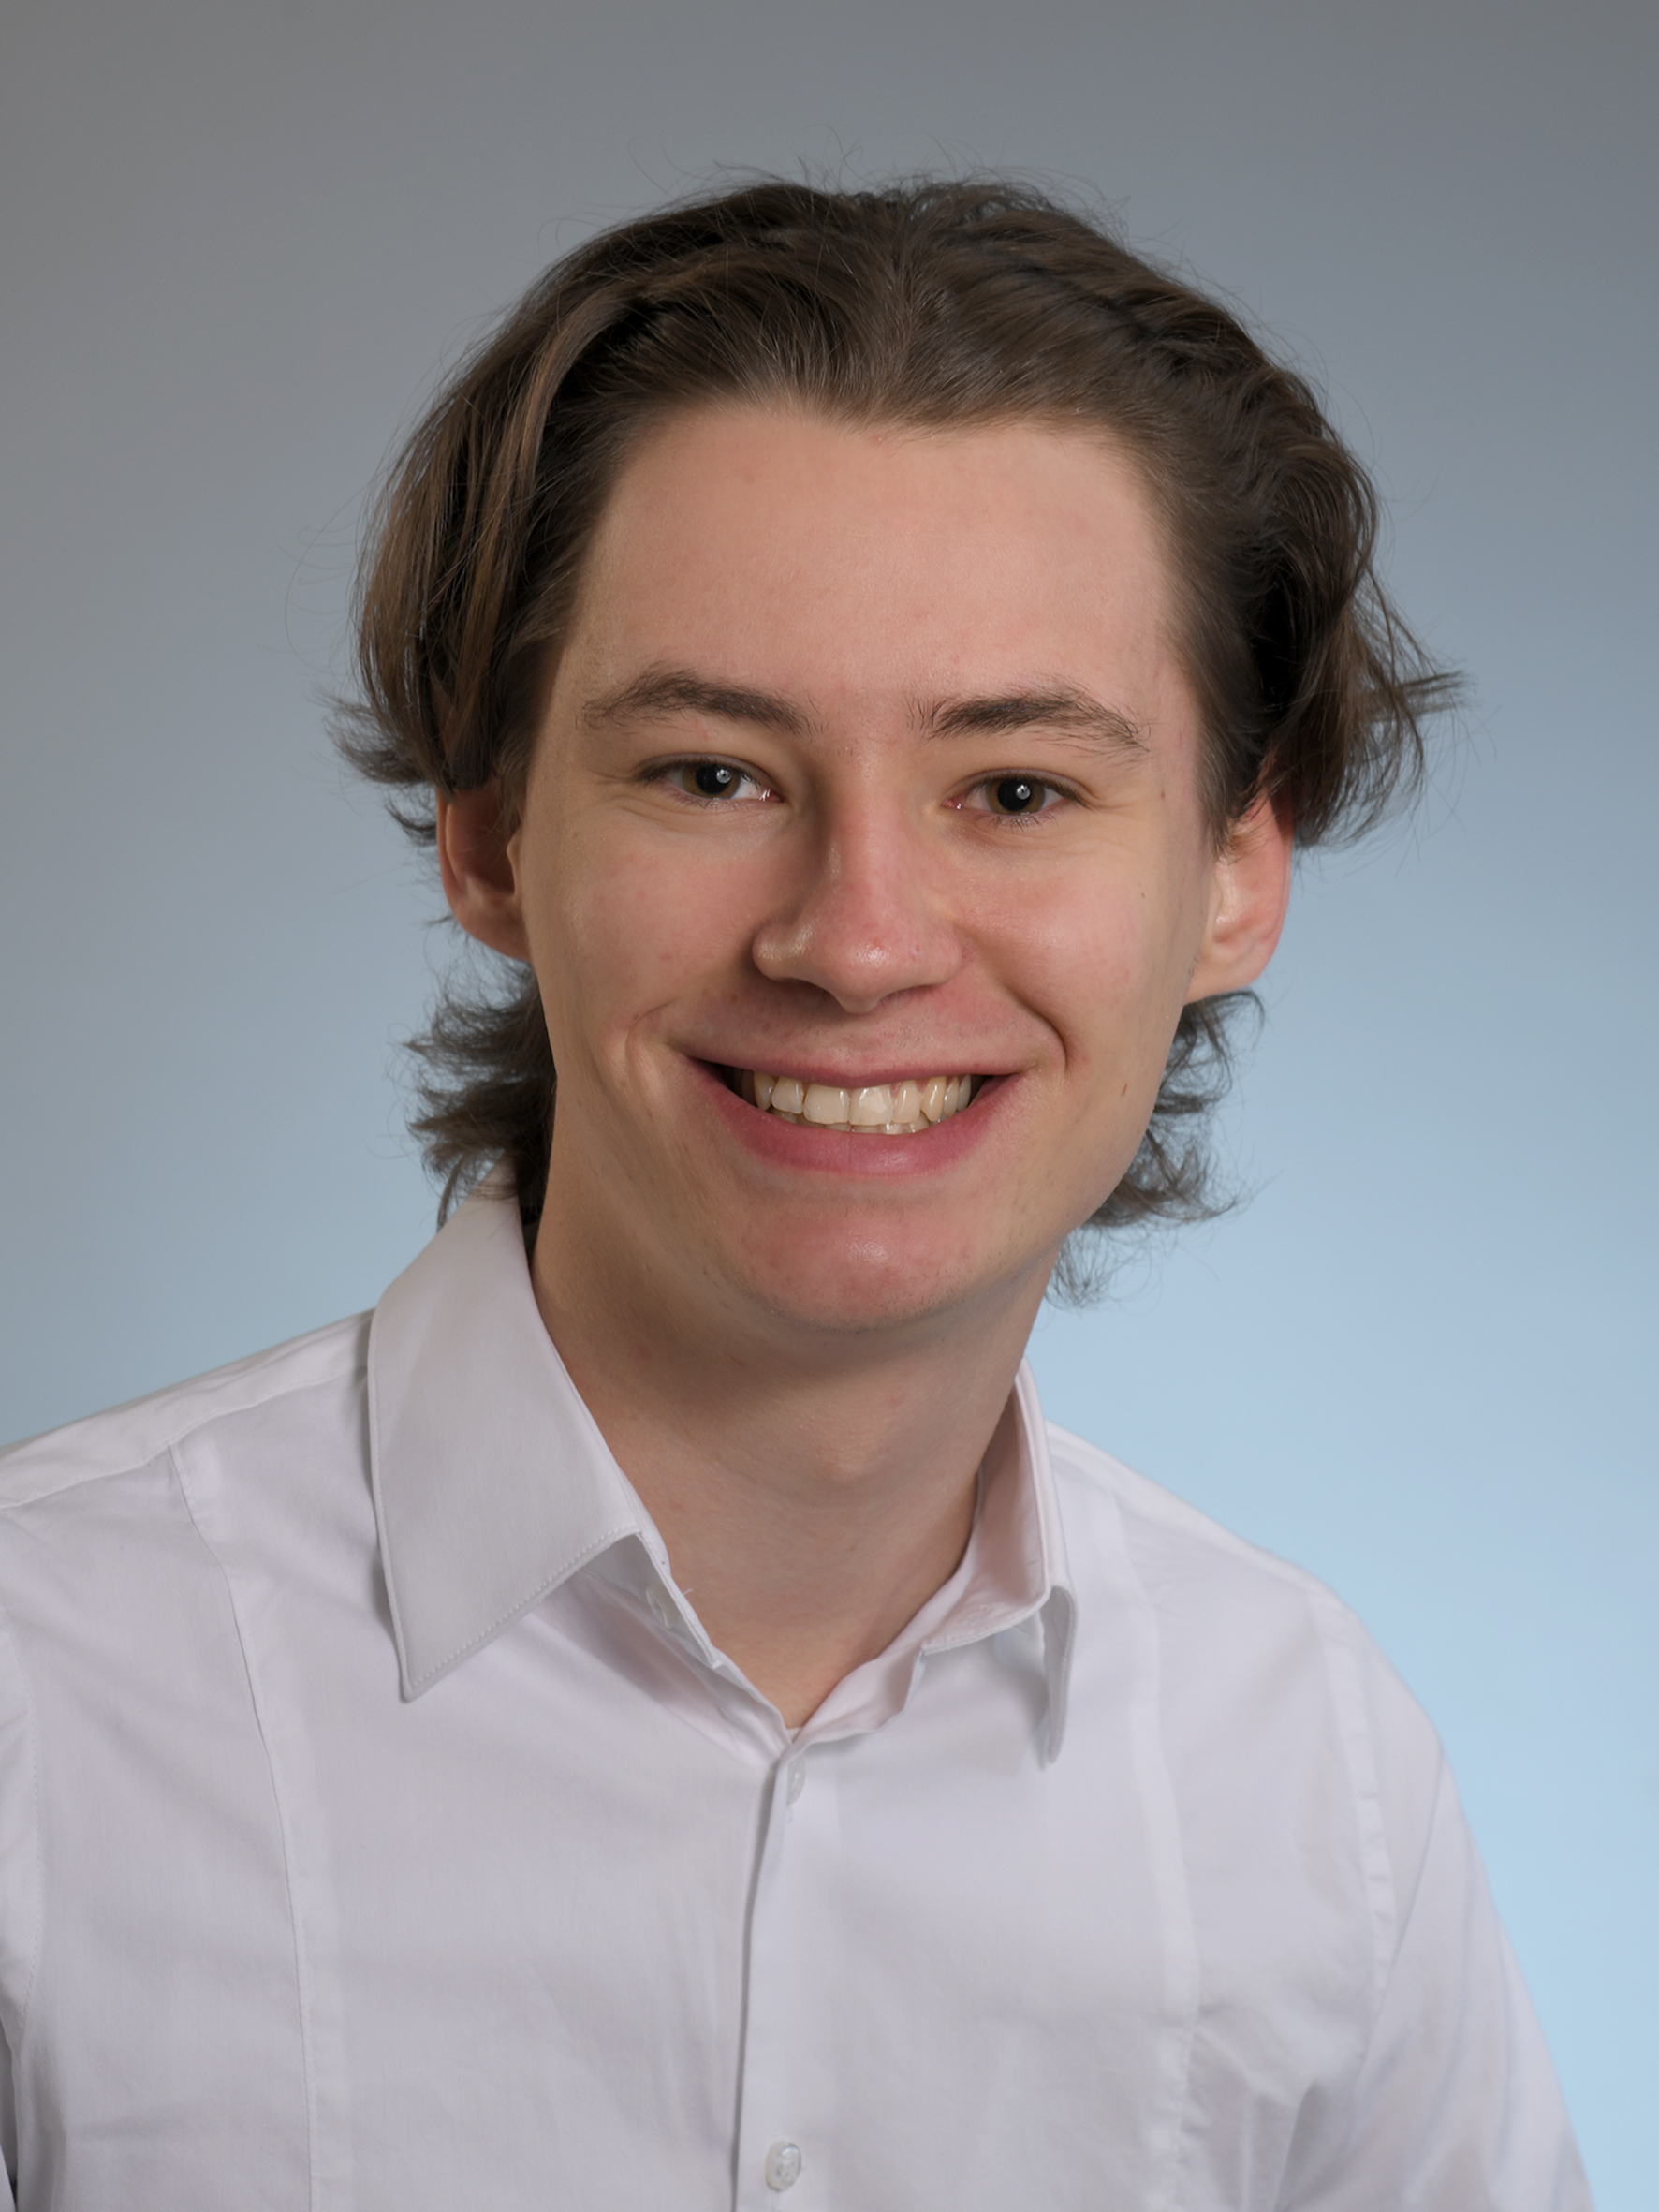
\includegraphics[width=\linewidth]{Fotoneu.jpg}	%trimming relative to image size

%---------------------------------------------------------------------------------------
%	META SKILLS
%----------------------------------------------------------------------------------------
\cvsection{SKILLS}

\cvskill{Deutsch} {1} \\[-2pt]

\cvskill{Englisch} {0.85} \\[-2pt]

\cvskill{Mathe} {0.55} \\[-2pt]

\cvskill{Python} {0.2} \\[-2pt]

\cvskill{HTML} {0.2} \\[-2pt]

\cvskill{Photoshop} {0.2} \\[-2pt]



\vfill\null
\cvsection{KONTAKT}
	
\icontext{MapMarker}{12}{Riedlen 25\\79353 Bahlingen}{black}\\[6pt]
\icontext{MobilePhone}{12}{+49 152 046 97 11 7}{black}\\[6pt]
\iconemail{Envelope}{12}{j@kob.one}{j@kob.one?subject=Einladung\%20zum\%20Vorstellungsgespr\%C3\%A4ch\&body=Wir\%20laden\%20Sie\%20herzlich\%20ein}{black}\\[6pt]
\iconhref{MousePointer}{12}{jakobenzo.github.io/classic-cv}{https://jakobenzo.github.io/classic-cv/}{black}\\[6pt]

\vfill\null
\cvqrcode{0.7}


%---------------------------------------------------------------------------------------
%	ABOUT ME
%----------------------------------------------------------------------------------------
\newpage
\cvsection{Über mich}

\aboutmemetaevent
{Ich bin 21 Jahre alt und interessiere mich sehr für Technik. In meiner Freizeit treffe ich meine Freunde Online oder auf dem Rasen. Seit knapp 19 Jahren spiele ich Fußball, und bin seit 13 Jahren aktives Mitglied im Fußballverein. Sofern es die Corona Regeln zulassen, bin ich gerne mit meinen Freunden im RealLife unterwegs. Meine Familie unterstütze ich unter anderem bei regelmäßigen Arbeitseinsätzen wie Holz machen oder Möbel schleppen. Mein Führerschein der Klasse A besitze ich seit knapp einem Jahr. IT News hole ich mir auf Reddit und gelegentlich bei heise.}

\vfill\null
\cvqrcode{0.7}


\end{leftcolumn}
\begin{rightcolumn}
%---------------------------------------------------------------------------------------
%	TITLE  HEADER
%----------------------------------------------------------------------------------------
\fcolorbox{white}{darkcol}{\begin{minipage}[c][3.5cm][c]{1\mpwidth}
	\begin {center}
		\HUGE{ \textbf{ \textcolor{white}{ \uppercase{JAKOB KAUFMANN} } } } \\[-24pt]
		\textcolor{white}{ \rule{0.1\textwidth}{1.25pt} } \\[4pt]
		\large{ \textcolor{white} {Ehrgeizig - Belastbar - Lernbegierig} }
	\end {center}
\end{minipage}} \\[14pt]
\vspace{-12pt}

%---------------------------------------------------------------------------------------
%	PROFILE
%----------------------------------------------------------------------------------------

\cvsection{Bewerbung}

\cvtext{Ich bewerbe mich für den Studienplatz \flqq Duales Studium Informatik \frqq\\

Gerne möchte ich bei Ihnen mein Studium absolvieren, um zu lernen, wie man Software nach modernen Standards entwickelt.
Die von Ihnen genannten Themenfelder decken ein breites Spektrum  ab, deren Einsatz in der Praxis ich gerne kennenlernen würde.\\

In der Oberstufe konnte ich erste Programmiererfahrung sammeln, dabei wurde mein Interesse an der Informatik geweckt.\\

Nach meinem FSJ habe ich mich 2021 für den Studiengang Informatik an Uni Freiburg eingeschrieben.
Dort habe ich erste Erfahrungen mit Python gesammelt. Leider konnte ich dort mein neu erlerntes Wissen nicht ausreichend in der Praxis umsetzen.\\

Deshalb habe ich mich dazu entschlossen, ein duales Informatikstudium zu absolvieren. Ich würde gerne bereits während des Studiums mein gelerntes Wissen produktiv anwenden.\\

Meine Stärken liegen in meiner schnellen Auffassungsgabe und in meiner Fähigkeit, Probleme kreativ zu lösen.\\
Englisch beherrsche ich in Wort und Schrift, und trotz meiner Note in Mathematik beherrsche ich mehr wie die Grundrechenarten und habe ein Verständnis für grundlegende Konzepte der Informatik. Probleme kann ich eigenständig lösen, und mir neues Wissen autodidaktisch aneignen.\\

Gerne bin ich dazu bereit vor Studienbeginn ein unbezahltes Praktikum zu absolvieren, um Sie von meinen Qualitäten zu überzeugen.\\

Ich freue mich, von Ihnen zu hören, und über Ihre Einladung zu einem persönlichen Gespräch.\\

Mit freundlichen Grüßen\\

Jakob Kaufmann\\


\includegraphics[width=3cm,height=1cm]{Unterschrift.jpg}	%trimming relative to image size 

}



%---------------------------------------------------------------------------------------
%	Ausbildung
%----------------------------------------------------------------------------------------
\newpage
\vfill\null
\cvsection{AUSBILDUNG}

\cvevent
	{Okt. 21 -  NOW}
	{Informatik Studium}
	{Albert-Ludwigs-Universität Freiburg}
	{2020 habe ich mein Informatikstudium an der Universität Freiburg begonnen. Vorlesungen mit Praxisbezug haben mir besonders gefallen.\\
An der Uni habe ich im Rahmen der Vorlesung \flqq Einführung in die Programmierung\frqq~Python erlernt.}

\vfill\null
\cvevent
	{Nov. 20 - Jun. 21}
	{FSJ}
	{Evangelische Kita am Weinberg Eichstetten}
	{Im Zuge meines  FSJ war ich Betreuer für eine körperlich eingeschränkte pädagogische Fachkraft. Zu zweit waren wir für eine komplette Gruppe von Kindergartenkindern verantwortlich. Ich wollte herausfinden, ob ich mir einen sozialen Beruf vorstellen kann. Die Betreuung der Kinder hat mir viel Freude bereitet, doch der Ruf der Informatik war stärker.}


\vfill\null
\cvevent
	{Sep. 17 - Jun. 20}
	{Wirtschaftsgymnasium}
	{Carl-Helbing-Schule Emmendingen}
	{In der Oberstufe wurde mein Interesse an der Informatik geweckt, dort habe ich die Basics verschiedenster Software kennengelernt, beispielsweise Greenfoot oder Photoshop.\\
            Ich war in der Klasse engagiert und habe von meinem Mitspracherecht Gebrauch gemacht.}


\vfill\null
\cvevent
	{Okt. 11 - Jul. 17}
	{Realschule}
	{Theodor-Frank-Realschule Teningen}
	{Während meiner Realschulzeit war ich mehrfach Teil der Schulmannschaft, das Team hat es bis zum Landesfinale geschafft. Mein Schulpraktikum habe ich im Einzelhandel und im Werkzeugbau absolviert.}
\vfill\null
\end{rightcolumn}
\end{paracol}
\end{document}

